%%%%%%%%%%%%%%%%%%%%%%%%%%%%%%%%%%%%%%%%%
% Beamer Presentation
% LaTeX Template
% Version 1.0 (10/11/12)
%
% This template has been downloaded from:
% http://www.LaTeXTemplates.com
%
% License:
% CC BY-NC-SA 3.0 (http://creativecommons.org/licenses/by-nc-sa/3.0/)
%
%%%%%%%%%%%%%%%%%%%%%%%%%%%%%%%%%%%%%%%%%

%----------------------------------------------------------------------------------------
%	PACKAGES AND THEMES
%----------------------------------------------------------------------------------------

\documentclass[UTF8,aspectratio=169,14pt]{ctexbeamer}

\usepackage{hyperref}
\hypersetup{
	colorlinks=true,
	linkcolor=red,
	anchorcolor=blue,
	citecolor=green
}

\mode<presentation> {
	
	% The Beamer class comes with a number of default slide themes
	% which change the colors and layouts of slides. Below this is a list
	% of all the themes, uncomment each in turn to see what they look like.
	
	%\usetheme{default}
	%\usetheme{AnnArbor}
	%\usetheme{Antibes}
	%\usetheme{Bergen}
	%\usetheme{Berkeley}
	%\usetheme{Berlin}
	%\usetheme{Boadilla}
	%\usetheme{CambridgeUS}
	%\usetheme{Copenhagen}
	%\usetheme{Darmstadt}
	%\usetheme{Dresden}
	%\usetheme{Frankfurt}
	%\usetheme{Goettingen}
	%\usetheme{Hannover}
	%\usetheme{Ilmenau}
	%\usetheme{JuanLesPins}
	%\usetheme{Luebeck}
	\usetheme{Madrid}
	%\usetheme{Malmoe}
	%\usetheme{Marburg}
	%\usetheme{Montpellier}
	%\usetheme{PaloAlto}
	%\usetheme{Pittsburgh}
	%\usetheme{Rochester}
	%\usetheme{Singapore}
	%\usetheme{Szeged}
	%\usetheme{Warsaw}
	
	% As well as themes, the Beamer class has a number of color themes
	% for any slide theme. Uncomment each of these in turn to see how it
	% changes the colors of your current slide theme.
	
	%\usecolortheme{albatross}
	%\usecolortheme{beaver}
	%\usecolortheme{beetle}
	%\usecolortheme{crane}
	%\usecolortheme{dolphin}
	%\usecolortheme{dove}
	%\usecolortheme{fly}
	%\usecolortheme{lily}
	%\usecolortheme{orchid}
	%\usecolortheme{rose}
	%\usecolortheme{seagull}
	%\usecolortheme{seahorse}
	%\usecolortheme{whale}
	%\usecolortheme{wolverine}
	
	%\setbeamertemplate{footline} % To remove the footer line in all slides uncomment this line
	%\setbeamertemplate{footline}[page number] % To replace the footer line in all slides with a simple slide count uncomment this line
	
	%\setbeamertemplate{navigation symbols}{} % To remove the navigation symbols from the bottom of all slides uncomment this line
}

\usepackage{graphicx} % Allows including images
\graphicspath{{./figs/}}
\usepackage{booktabs} % Allows the use of \toprule, \midrule and \bottomrule in tables
\usepackage{longtable}
\usepackage{listings}
\usepackage{xcolor}
\lstset{numbers=left, %设置行号位置
	numberstyle=\tiny, %设置行号大小
	keywordstyle=\color{blue}, %设置关键字颜色
	commentstyle=\color[cmyk]{1,0,1,0}, %设置注释颜色
	frame=single, %设置边框格式
	escapeinside=``, %逃逸字符(1左面的键),用于显示中文
	%breaklines, %自动折行
	extendedchars=false, %解决代码跨页时,章节标题,页眉等汉字不显示的问题
	xleftmargin=2em,xrightmargin=2em, aboveskip=1em, %设置边距
	tabsize=4, %设置tab空格数
	showspaces=false %不显示空格
}
% Fonts
% \usepackage{libertine}
% \setmonofont{Courier}
\setCJKsansfont[ItalicFont=Noto Serif CJK SC Black, BoldFont=Noto Sans CJK SC Black]{Noto Sans CJK SC}


%----------------------------------------------------------------------------------------
%	TITLE PAGE
%----------------------------------------------------------------------------------------

\title[第3讲]{第3讲 中断、异常和系统调用} % The short title appears at the bottom of every slide, the full title is only on the title page
\subtitle{第一节:中断的概念}
\author{向勇、陈渝} % Your name
\institute[清华大学] % Your institution as it will appear on the bottom of every slide, may be shorthand to save space
{
清华大学计算机系 \\ % Your institution for the title page
\medskip
\textit{xyong,yuchen@tsinghua.edu.cn} % Your email address
}
\date{\today} % Date, can be changed to a custom date

\begin{document}

\begin{frame}
\titlepage % Print the title page as the first slide
\end{frame}

%----------------------------------------------------------------------------------------
\begin{frame}
\frametitle{提纲} % Table of contents slide, comment this block out to remove it
\tableofcontents % Throughout your presentation, if you choose to use \section{} and \subsection{} commands, these will automatically be printed on this slide as an overview of your presentation
\end{frame}

%----------------------------------------------------------------------------------------
%	PRESENTATION SLIDES
%----------------------------------------------------------------------------------------
%------------------------------------------------
\section{第一节:中断的概念}% Sections can be created in order to organize your presentation into discrete blocks, all sections and subsections are automatically printed in the table of contents as an overview of the talk
%------------------------------------------------

\subsection{背景} % A subsection can be created just before a set of slides with a common theme to further break down your presentation into chunks
%------------------------------------------------
\begin{frame}
	\frametitle{背景}
%	\framesubtitle{xxxx}
    \begin{itemize}
        \item 为什么需要中断、异常和系统调用
        \begin{itemize}
            \item 在计算机运行中,内核是被信任的第三方
            \item 只有内核可以执行特权指令
            \item 方便应用程序
        \end{itemize}
        \item 中断和异常希望解决的问题
        \begin{itemize}
            \item 当外设连接计算机时,会出现什么现象?
            \item 当应用程序处理意想不到的行为时,会出现什么现象?
        \end{itemize}
        \item 系统调用希望解决的问题
        \begin{itemize}
            \item 用户应用程序是如何得到系统服务?
            \item 系统调用和功能调用的不同之处是什么?
        \end{itemize}
    \end{itemize}
\end{frame}
%------------------------------------------------
\begin{frame}
	\frametitle{计算机体系结构概述}
%	\framesubtitle{xxxx}
\begin{figure}
    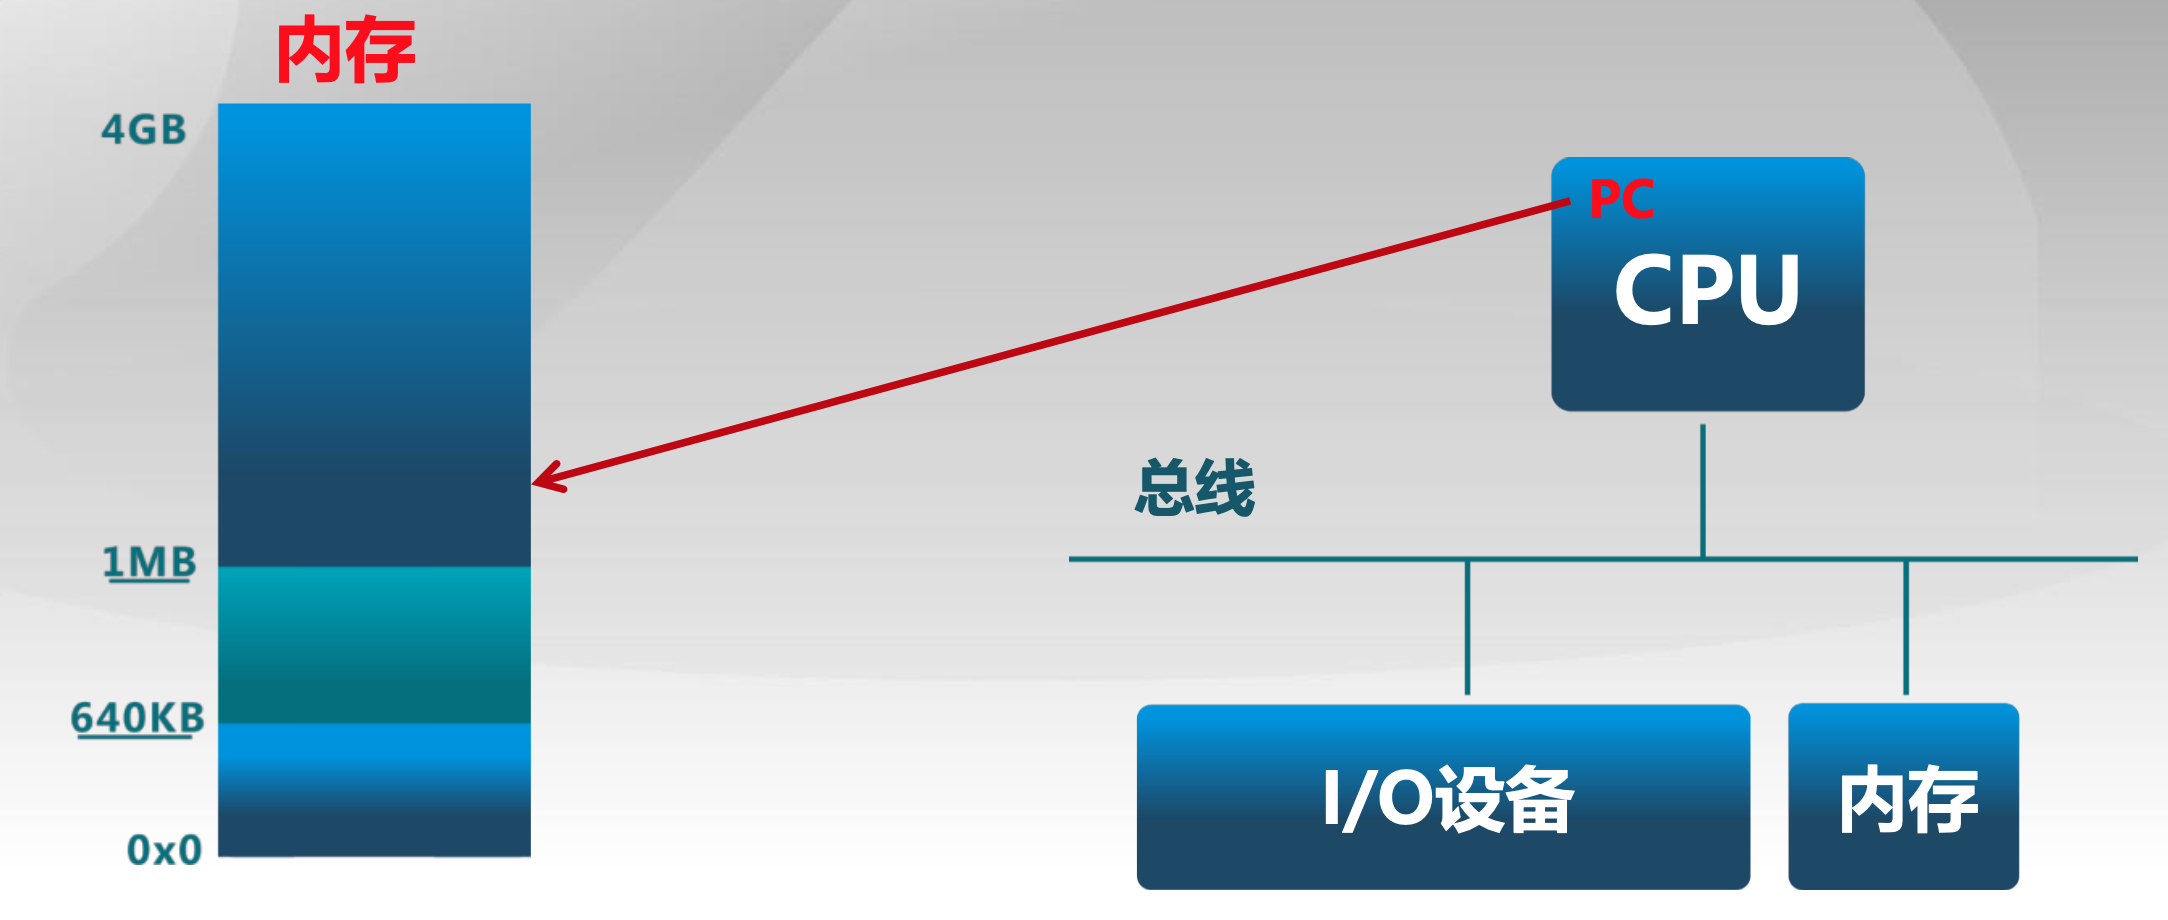
\includegraphics[width=1.0\linewidth]{architecture}
\end{figure}

\end{frame}
% 2018-lec3-chy.pdf:P3、P4
% 
%------------------------------------------------
\begin{frame}
	\frametitle{SiFive FE310-G002 top-level block diagram}
%	\framesubtitle{xxxx}
\begin{figure}
    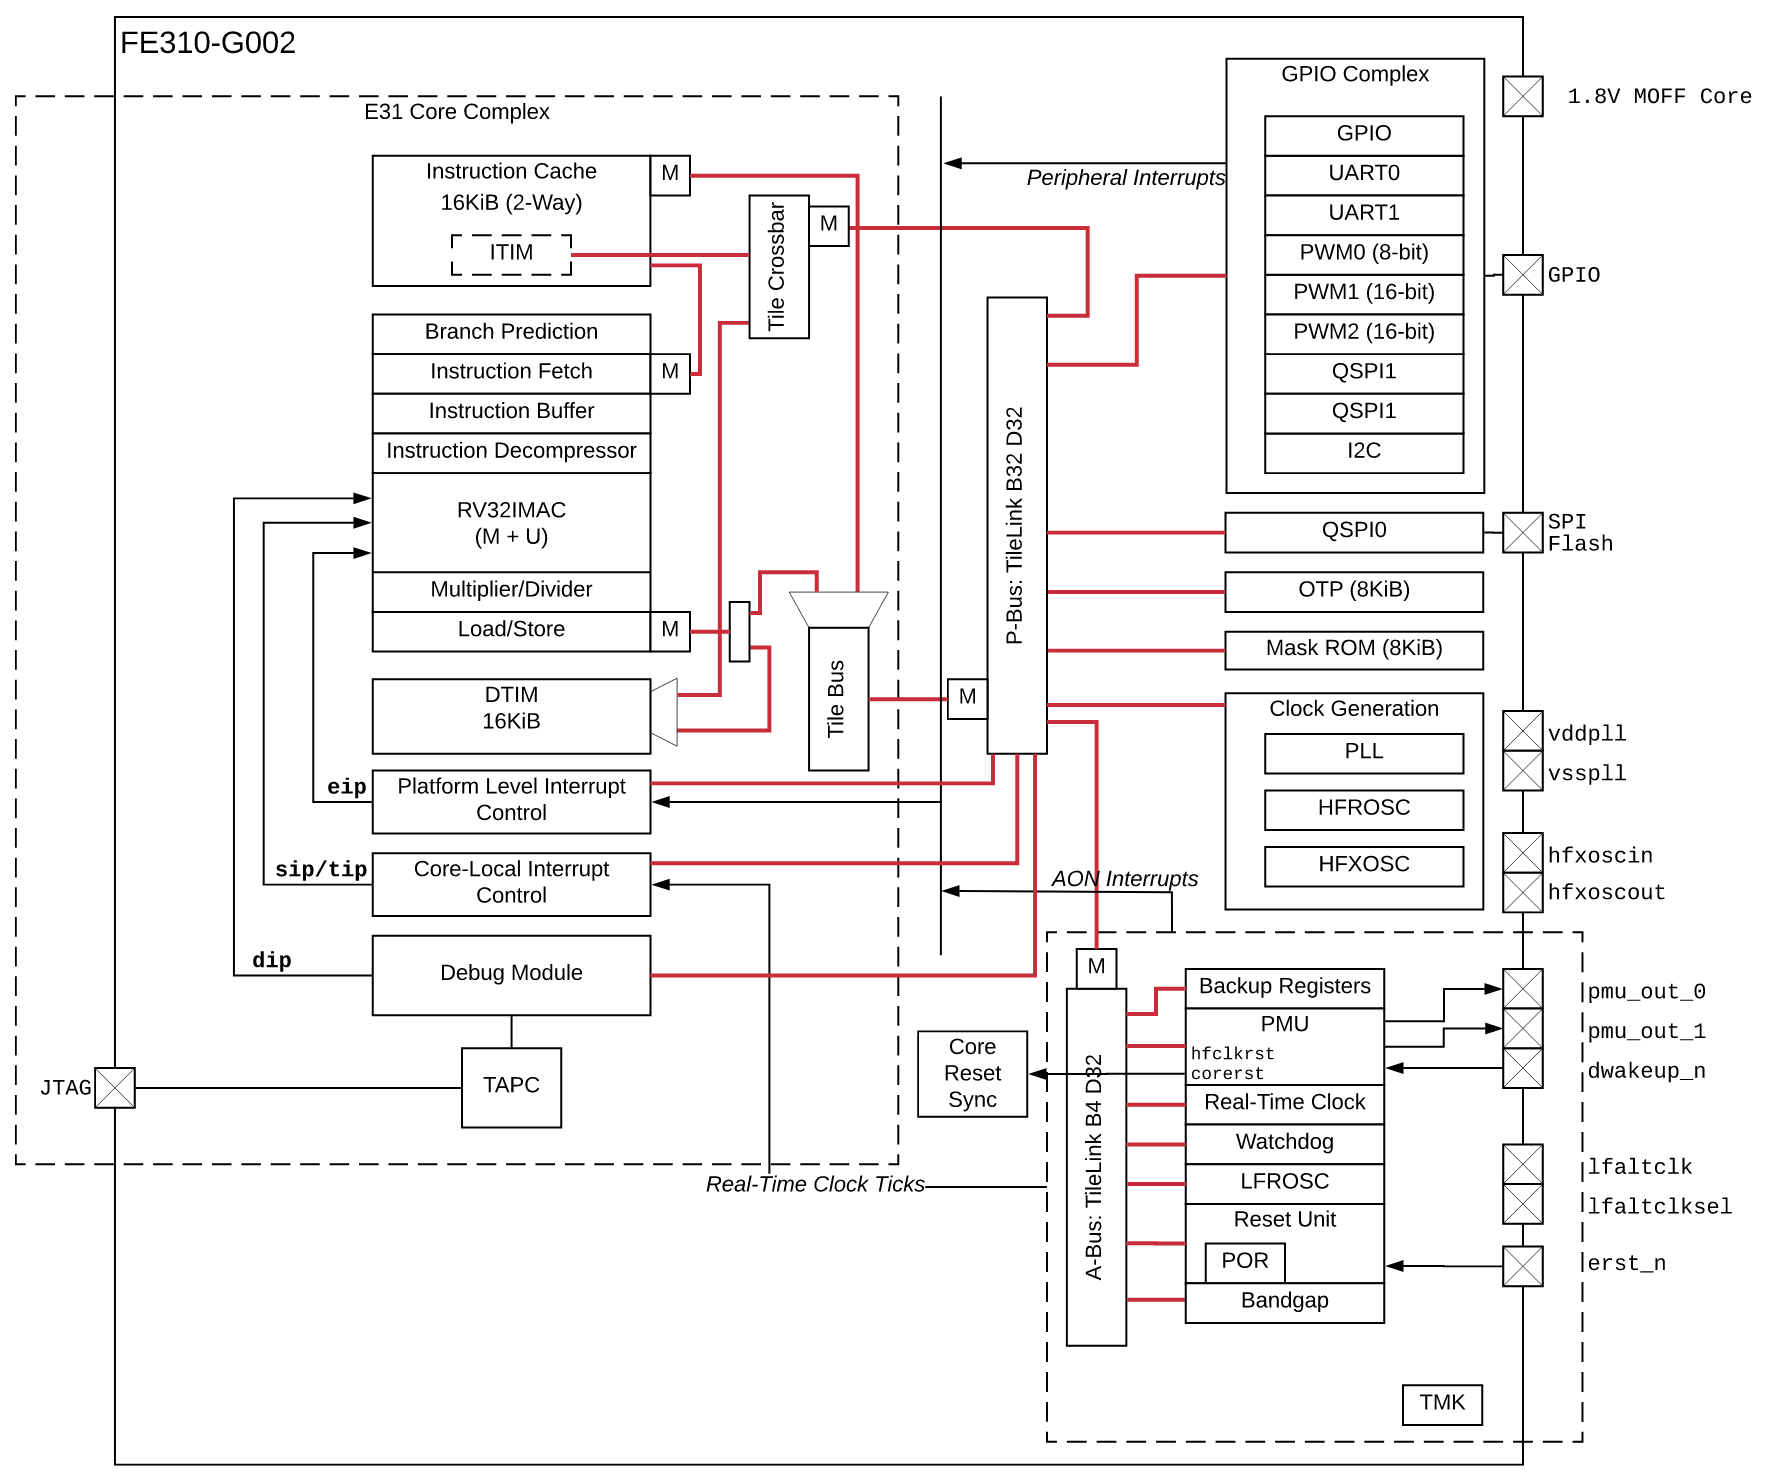
\includegraphics[width=1.0\linewidth]{sifive-board}
\end{figure}
\end{frame}
% https://cdn.sparkfun.com/assets/5/b/e/6/2/fe310-g002-ds.pdf
%------------------------------------------------
% #### RV板级图
% 
% 需要补充(类似2018-lec3-chy.pdf:P9)
% 
%------------------------------------------------
\subsection{内核的进入与退出}
%------------------------------------------------
\begin{frame}
	\frametitle{xxxx}
	\framesubtitle{xxxx}
\end{frame}

%------------------------------------------------
% ### 内核的进入与退出
% 
% #### 内核的进入与退出
% 
% 2018-lec3-chy.pdf:P31
% 插图
% 

%------------------------------------------------
\subsection{中断、异常和系统调用}
%------------------------------------------------
\begin{frame}
	\frametitle{xxxx}
	\framesubtitle{xxxx}
\end{frame}

%------------------------------------------------
% ### 中断、异常和系统调用
% 
% #### 中断、异常和系统调用
% 
% 2018-lec3-chy.pdf:P25
% 源头
% 	中断:外设
% 	异常:应用程序意想不到的行为
% 	系统调用:应用程序请求操作提供服务
% 响应方式
% 	中断:异步
% 	异常:同步
% 	系统调用:异步或同步
% 处理机制
% 	中断:持续,对用户应用程序是透明的
% 	异常:杀死或者重新执行意想不到的应用程序指令
% 	系统调用:等待和持续
% 
%------------------------------------------------
\begin{frame}
	\frametitle{xxxx}
	\framesubtitle{xxxx}
\end{frame}
%------------------------------------------------
% #### 中断向量
% ref:
% rv的中断编号
% 
%------------------------------------------------
\begin{frame}
	\frametitle{xxxx}
	\framesubtitle{xxxx}
\end{frame}
%------------------------------------------------
% #### 中断、异常和系统调用比较
% 
% 插图2018-lec3-chy.pdf:P32
% 
% 源头
% 	中断:外设
% 	异常:应用程序意想不到的行为
% 	系统调用:应用程序请求操作提供服务
% 响应方式
% 	中断:异步
% 	异常:同步
% 	系统调用:异步或同步
% 处理机制
% 	中断:持续,对用户应用程序是透明的
% 	异常:杀死或者重新执行意想不到的应用程序指令
% 	系统调用:等待和持续
% 
%------------------------------------------------
\begin{frame}
	\frametitle{xxxx}
	\framesubtitle{xxxx}
\end{frame}
%------------------------------------------------
% #### 中断、异常和系统调用的用途
% 2018-lec3-chy.pdf:P33
% 系统调用(system call)
% 	应用程序主动向操作系统发出的服务请求
% 异常(exception)
% 	非法指令或者其他原因导致当前指令执行失败 (如:内存出错)后的处理请求
% 中断(hardware interrupt)
% 	来自硬件设备的处理请求
% 

%------------------------------------------------
\subsection{中断处理机制}

%------------------------------------------------
\begin{frame}
	\frametitle{xxxx}
	\framesubtitle{xxxx}
\end{frame}
%------------------------------------------------
% ### 中断处理
% 
% #### 中断处理-硬件
% 
% 插图2018-lec3-chy.pdf:P34
% 
% 硬件处理
% 在CPU初始化时设置中断使能标志
% 	依据内部或外部事件设置中断标志
% 	依据中断向量调用相应中断服务例程
% 
%------------------------------------------------
\begin{frame}
	\frametitle{xxxx}
	\framesubtitle{xxxx}
\end{frame}
%------------------------------------------------
% #### 中断处理-软件
% 
% 插图2018-lec3-chy.pdf:P35
% 
% 软件
% 现场保存(CPU+编译器)
% 中断服务处理(服务例程)
% 清除中断标记(服务例程)
% 现场恢复(CPU+编译器)
% 
%------------------------------------------------
\begin{frame}
	\frametitle{xxxx}
	\framesubtitle{xxxx}
\end{frame}
%------------------------------------------------
% #### 中断嵌套
% 2018-lec3-chy.pdf:P36
% 硬件中断服务例程可被打断
% 	不同硬件中断源可能在硬件中断处理时出现
% 	硬件中断服务例程中需要临时禁止中断请求
% 	中断请求会保持到CPU做出响应
% 异常服务例程可被打断
% 	异常服务例程执行时可能出现硬件中断
% 异常服务例程可嵌套
% 	异常服务例程可能出现缺页
%----------------------------------------------------------------------------------------

\end{document}
